\documentclass[11pt,a4paper]{article} 
\usepackage{subcaption}
\usepackage{graphicx} % Required for inserting images
\usepackage{booktabs}
\usepackage{enumerate}
\usepackage{float}
\usepackage[table,xcdraw]{xcolor}
\usepackage[left=2.5cm, right=2.5cm]{geometry}
\usepackage{natbib}


\title{EDA Summative Assessment} 
\author{Isaac Beight-Welland} 
\date{March 2023} 

\newcommand{\bold}[1]{\textbf{#1}} \newcommand{\ital}[1]{\textit{#1}}
\newcommand{\formula}[1]{\small\texttt{#1}\normalsize}
\newcommand{\itemspace}{\vspace{1em}\item}
\newcommand{\parspace}{\par\vspace{1em}}

\begin{document}

\maketitle



\section*{Question 1.1}



\begin{enumerate}[a)] 

  \itemspace 
    
    \ital{How would you characterise the design (cross-section, repeated
    cross-section, panel, time-series...) of the “European Values Study”?} \par

    The European Values Study is a repeated cross-sectional survey as a
    different samples are used between the different time periods: the sample
    from the first year is different from the next. 
    
  \itemspace 

    \ital{Is the source of the data experimental or observational?} \par

    I would argue that the European Values Study as a survery is observational
    as it does not discriminate between a treatment and control group. Instead
    observations are made by comparing associations between answers of
    different respondants, this makes it more difficult to discern a causation. \par

  \itemspace 

    \ital{Life satisfaction and Employment are self-reported variables. What
    does “self-reported” mean? Explain why self-reported variables might create
    issues in terms of the accuracy and comparability of the data.} \par

    Self-reported variables ask participants to measure themselves, this can
    create issues with data validity as participants may not be honest, or
    their experiences may impact the severity of their response despite having
    similar circumstances to others. \par
    
  \itemspace 

    \ital{How would you interpret a value higher than 90 for the variable
    percentile? Briefly explain why the variable percentile is better suited
    than the absolute level of income (Monthly household income) to compare
    individuals at different points of the income distribution and across
    countries.} \par 

    A value higher than 90 means that the absolute value of the variable is in
    the top 10\% of the total sample. In terms of monthly household income, a
    value of 90 would indicate that they have an individiaul income greater
    than 90\% of the country population's incomes.
    
  \itemspace 

    \ital{The variable Full employment is constructed from the variable
    Employment with the following formula:} \par 
    
    \begin{center}
    \formula{=IF(OR(R2="Full time", R2="Unemployed"), IF(R2="Full
    time",1,0),"")} 
    \end{center}\par
    
    \ital{Where R is the column for Employment, Explain how the formula works.
    What is the value returned for an individual who only works part time?} \par 

    The formula consists of a nested if statement. First it checks whether the
    variable is "Full time" or "Unemployed", if so, the values 1 and 0 are
    applied respectively. If the value is neither of the two (as indicated by
    the OR operator), then the value remains blank "". 

\end{enumerate}



\newpage
\section*{Question 1.2}



\begin{table}[h!]

\resizebox{\textwidth}{!}{%
\begin{tabular}{@{}llllll@{}}
\rowcolor[HTML]{D9D9D9} 
\textbf{Row Labels}  & \textbf{Respondant count}     & \textbf{Life sat. Mean} & \textbf{Life sat. StdDev} & \textbf{Work eth. Mean} & \textbf{Work eth. StdDev} \\ \midrule
Albania            & 1200 & 6.471 & 2.263 & 3.923 & 0.610 \\
Armenia            & 1224 & 5.705 & 2.586 & 3.886 & 0.636 \\
Austria            & 1216 & 7.476 & 2.100 & 3.723 & 0.756 \\
Belarus            & 1237 & 6.065 & 2.078 & 3.620 & 0.761 \\
Bosnia Herzegovina & 1104 & 7.084 & 2.364 & 3.545 & 0.657 \\
Bulgaria           & 1183 & 5.705 & 2.737 & 4.117 & 0.625 \\
Croatia            & 1188 & 7.071 & 2.359 & 3.406 & 0.718 \\
Cyprus             & 775  & 7.209 & 2.194 & 4.065 & 0.700 \\
Czech Republic     & 1308 & 7.192 & 2.091 & 3.633 & 0.781 \\
Denmark            & 1061 & 8.408 & 1.769 & 3.537 & 0.736 \\
Estonia            & 1273 & 6.619 & 2.135 & 3.550 & 0.757 \\
Finland            & 940  & 7.714 & 1.794 & 3.273 & 0.784 \\
Georgia            & 1233 & 5.486 & 2.464 & 3.994 & 0.641 \\
Greece             & 1246 & 6.921 & 2.235 & 3.817 & 0.723 \\
Hungary            & 1248 & 6.295 & 2.318 & 3.852 & 0.663 \\
Iceland            & 666  & 8.072 & 1.612 & 2.808 & 0.683 \\
Ireland            & 504  & 7.823 & 1.658 & 3.473 & 0.825 \\
Italy              & 876  & 7.398 & 2.046 & 3.734 & 0.712 \\
Kosovo             & 1339 & 6.839 & 2.547 & 4.073 & 0.654 \\
Latvia             & 1197 & 6.347 & 2.082 & 3.498 & 0.615 \\
Lithuania          & 1143 & 6.303 & 2.258 & 3.557 & 0.590 \\
Luxembourg         & 1165 & 7.833 & 2.063 & 3.683 & 0.835 \\
Macedonia          & 1290 & 6.933 & 2.400 & 3.846 & 0.750 \\
Malta              & 730  & 7.685 & 2.142 & 3.541 & 0.649 \\
Moldova            & 1174 & 6.563 & 2.532 & 3.898 & 0.596 \\
Montenegro         & 1166 & 7.581 & 2.322 & 3.708 & 0.773 \\
Netherlands        & 1250 & 7.990 & 1.213 & 3.148 & 0.753 \\
Northern Cyprus    & 404  & 6.386 & 2.501 & 3.879 & 0.542 \\
Northern Ireland   & 309  & 7.819 & 1.579 & 3.313 & 0.681 \\
Norway             & 992  & 8.104 & 1.679 & 3.580 & 0.768 \\
Poland             & 1050 & 7.216 & 1.962 & 3.496 & 0.638 \\
Portugal           & 764  & 6.372 & 2.024 & 3.898 & 0.616 \\
Romania            & 1025 & 6.899 & 2.473 & 3.871 & 0.682 \\
Russian Federation & 1102 & 6.524 & 2.432 & 3.621 & 0.763 \\
Serbia             & 1216 & 6.932 & 2.404 & 3.665 & 0.702 \\
Slovakia           & 1042 & 7.055 & 2.182 & 3.833 & 0.761 \\
Slovenia           & 801  & 7.623 & 1.988 & 3.682 & 0.654 \\
Sweden             & 788  & 7.679 & 2.074 & 3.247 & 0.773 \\
Switzerland        & 934  & 7.968 & 1.773 & 3.450 & 0.690 \\
Ukraine            & 1178 & 6.010 & 2.446 & 3.737 & 0.748 \\
\rowcolor[HTML]{D9D9D9} 
\textbf{Grand Total} & \textbf{41541} & \textbf{6.965}                  &
\textbf{2.318}                    & \textbf{3.674}           & \textbf{0.748}
\\ \end{tabular}%
}
\caption{Shows averages and standard deviation for Life Satisfaction and Work
  Ethic by country for wave 4.}
\label{tab:Q1_2}
\end{table}  

\noindent As shown in Table \ref{tab:Q1_2} there are 39 countries that are
represented in wave 4. Furthermore, there are a total of 41541 respondants for
wave 4. \parspace

\noindent There is a higher average life satisfaction in Iceland (8.072) than in Italy
(7.398) and a smaller standard deviation, 1.612 compared to 2.046. Since both
the average responses is greater, and there is less deviation between
responses, it could be argued that individuals are generally happier in Iceland
compared to Italy. Furthermore, life satisfaction itself is not a measurement of
happiness \citep{happiness}. It is possible that a person is satisfied with
their life, for example, satisfied with their life achievements, families,
relationships, etc. but not happy as of itself. 

\noindent Since Iceland had a lesser average response to the work ethic question, 2.808 compared to 3.734, it could be argued that unemployed individuals in Italy are more likely to be stigmatised for not working than in Iceland since the society values work more. 

\newpage
\section*{Question 1.3}



\begin{figure}[h]
  \begin{center}
    \begin{subfigure}{0.49\textwidth}
      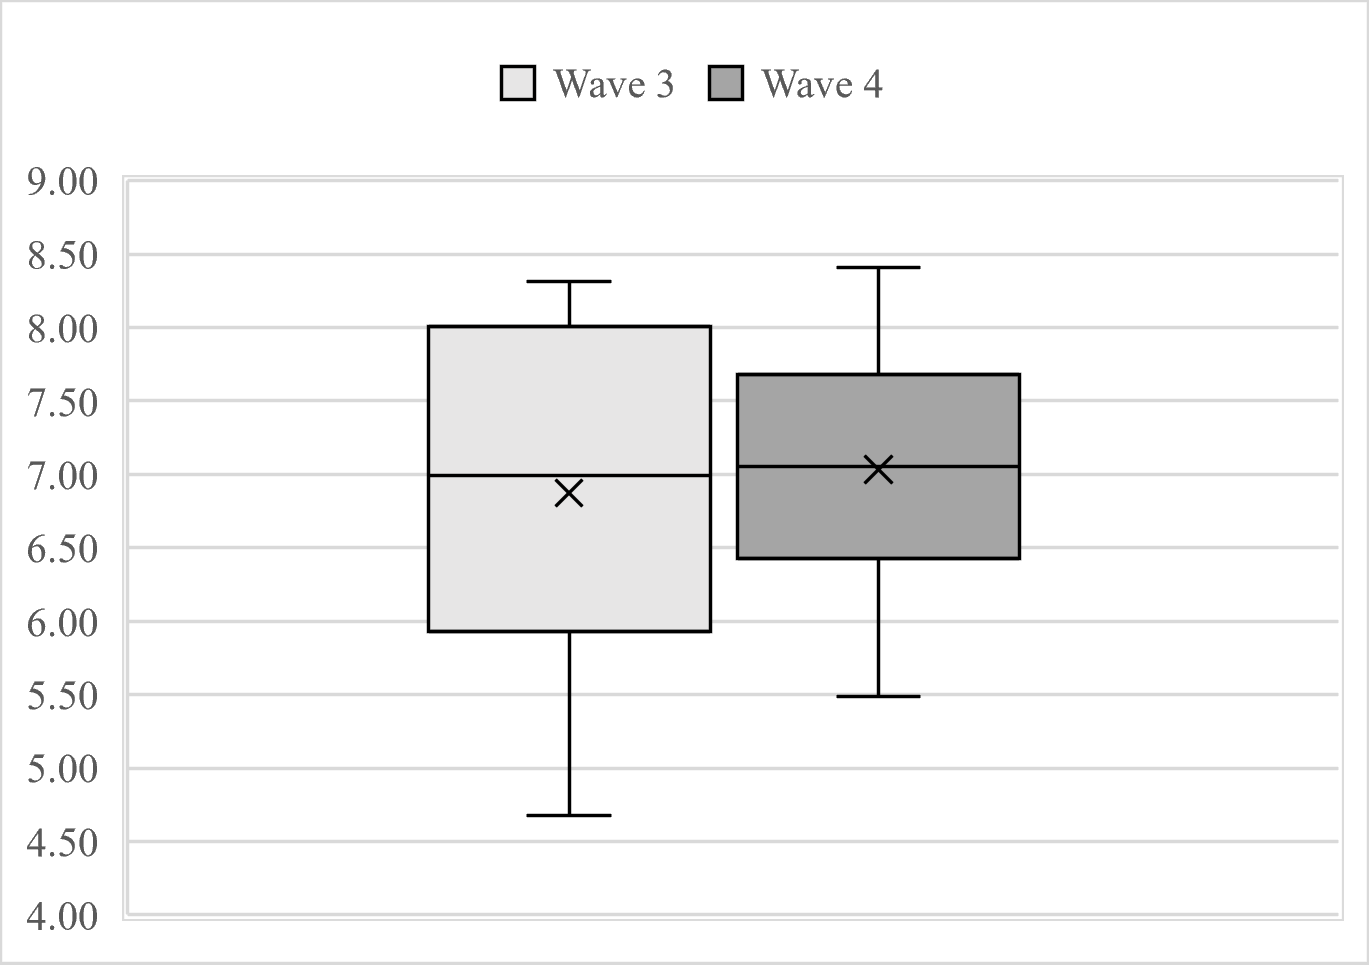
\includegraphics[width=0.95\linewidth]{figures/LifeSatisfactionQ1_3.png}
      \caption{Life Satisfaction}
      \label{fig:LifeSatisfactionQ1_3}
    \end{subfigure}
    \begin{subfigure}{0.49\textwidth}
      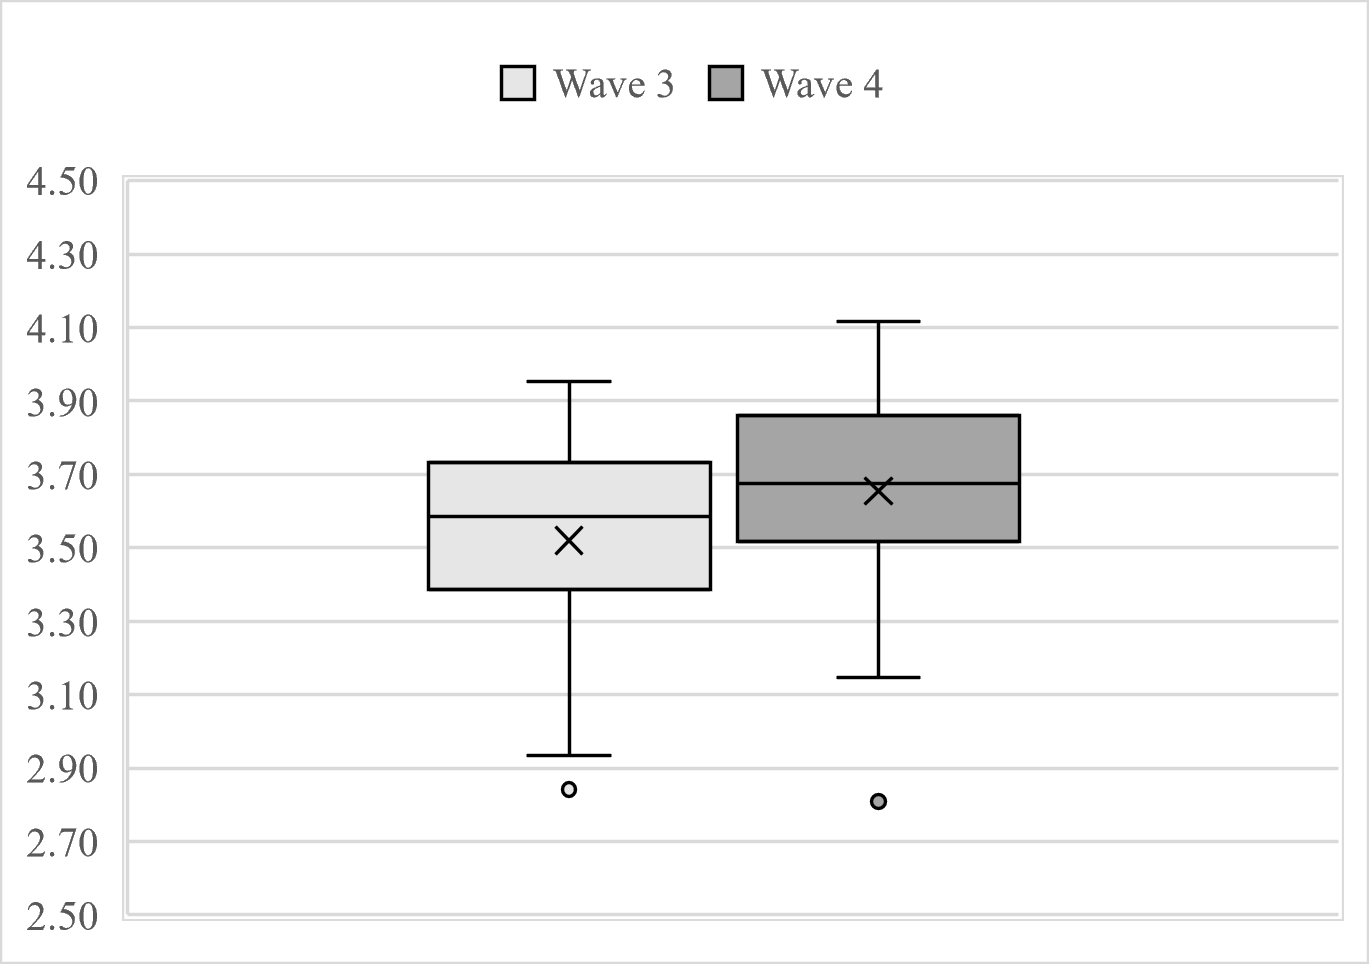
\includegraphics[width=0.95\linewidth]{figures/WorkEthicQ1_3.png}
      \caption{Work Ethic}
      \label{fig:WorthEthicQ1_3}
    \end{subfigure}
  \end{center}
  \caption{Avera}
  \label{fig:Q1_3}
\end{figure}



\newpage
\section*{Question 1.4}



\begin{figure}[h]
  \begin{center}
    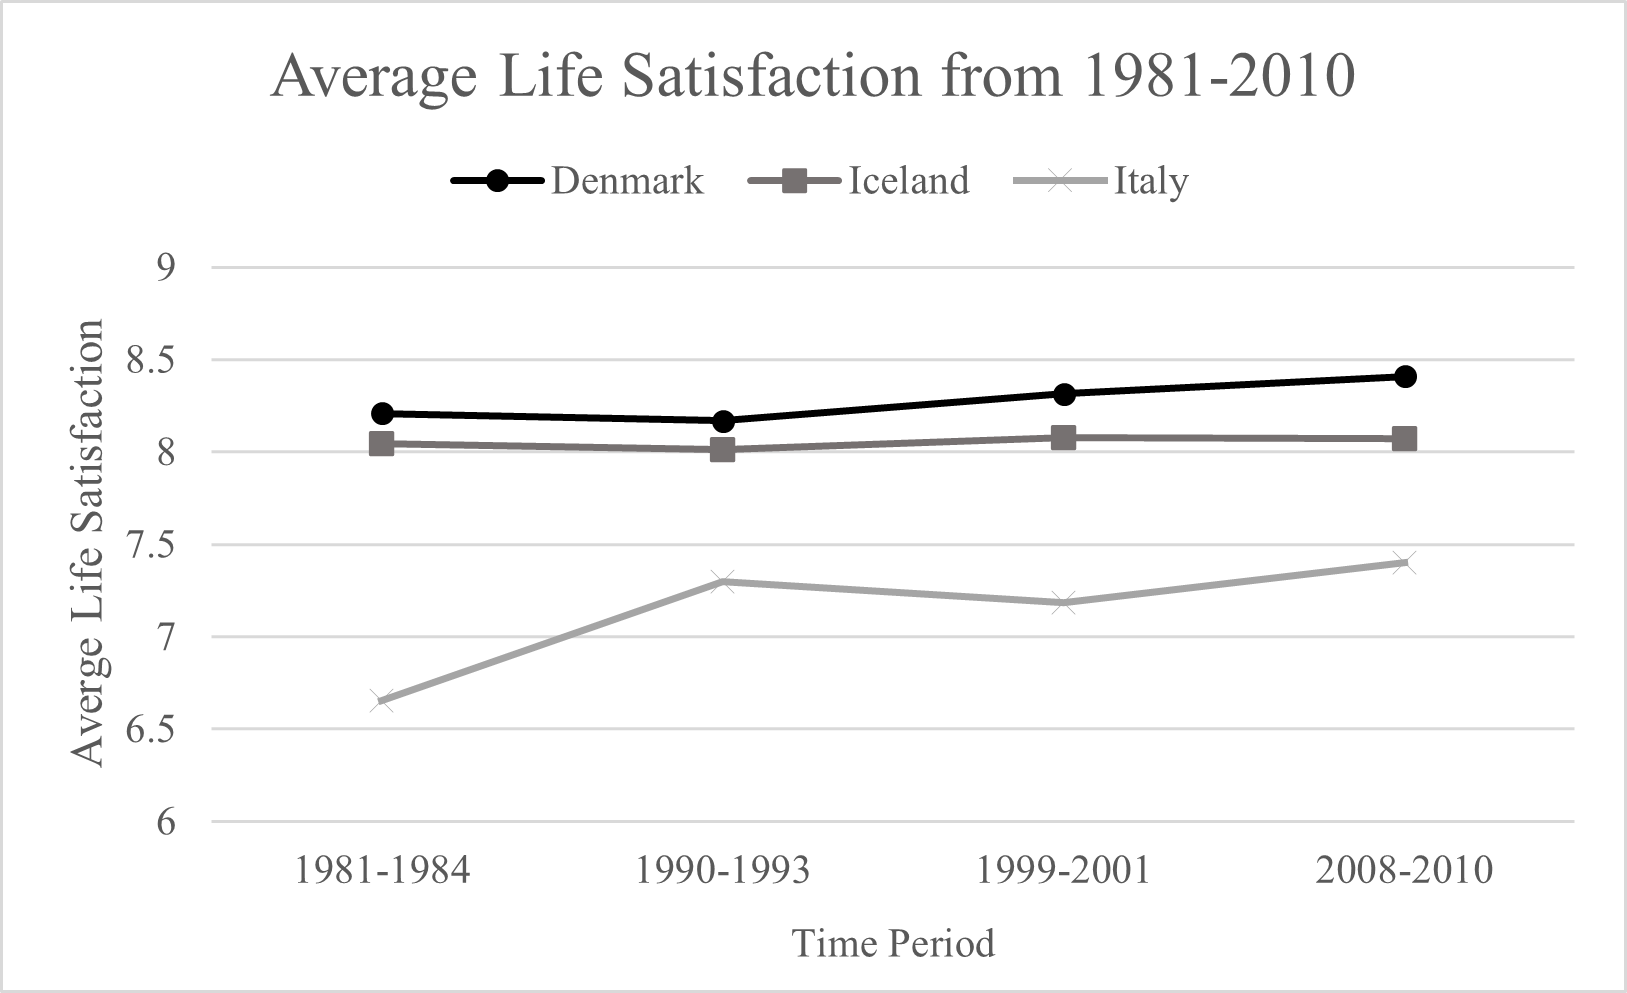
\includegraphics[width=0.95\textwidth]{figures/Q1_4.png}
  \end{center}
  \caption{}
  \label{fig:Q1_4}
\end{figure}



\newpage
\section*{Question 1.5}



\begin{figure}[H]
  \begin{center}
    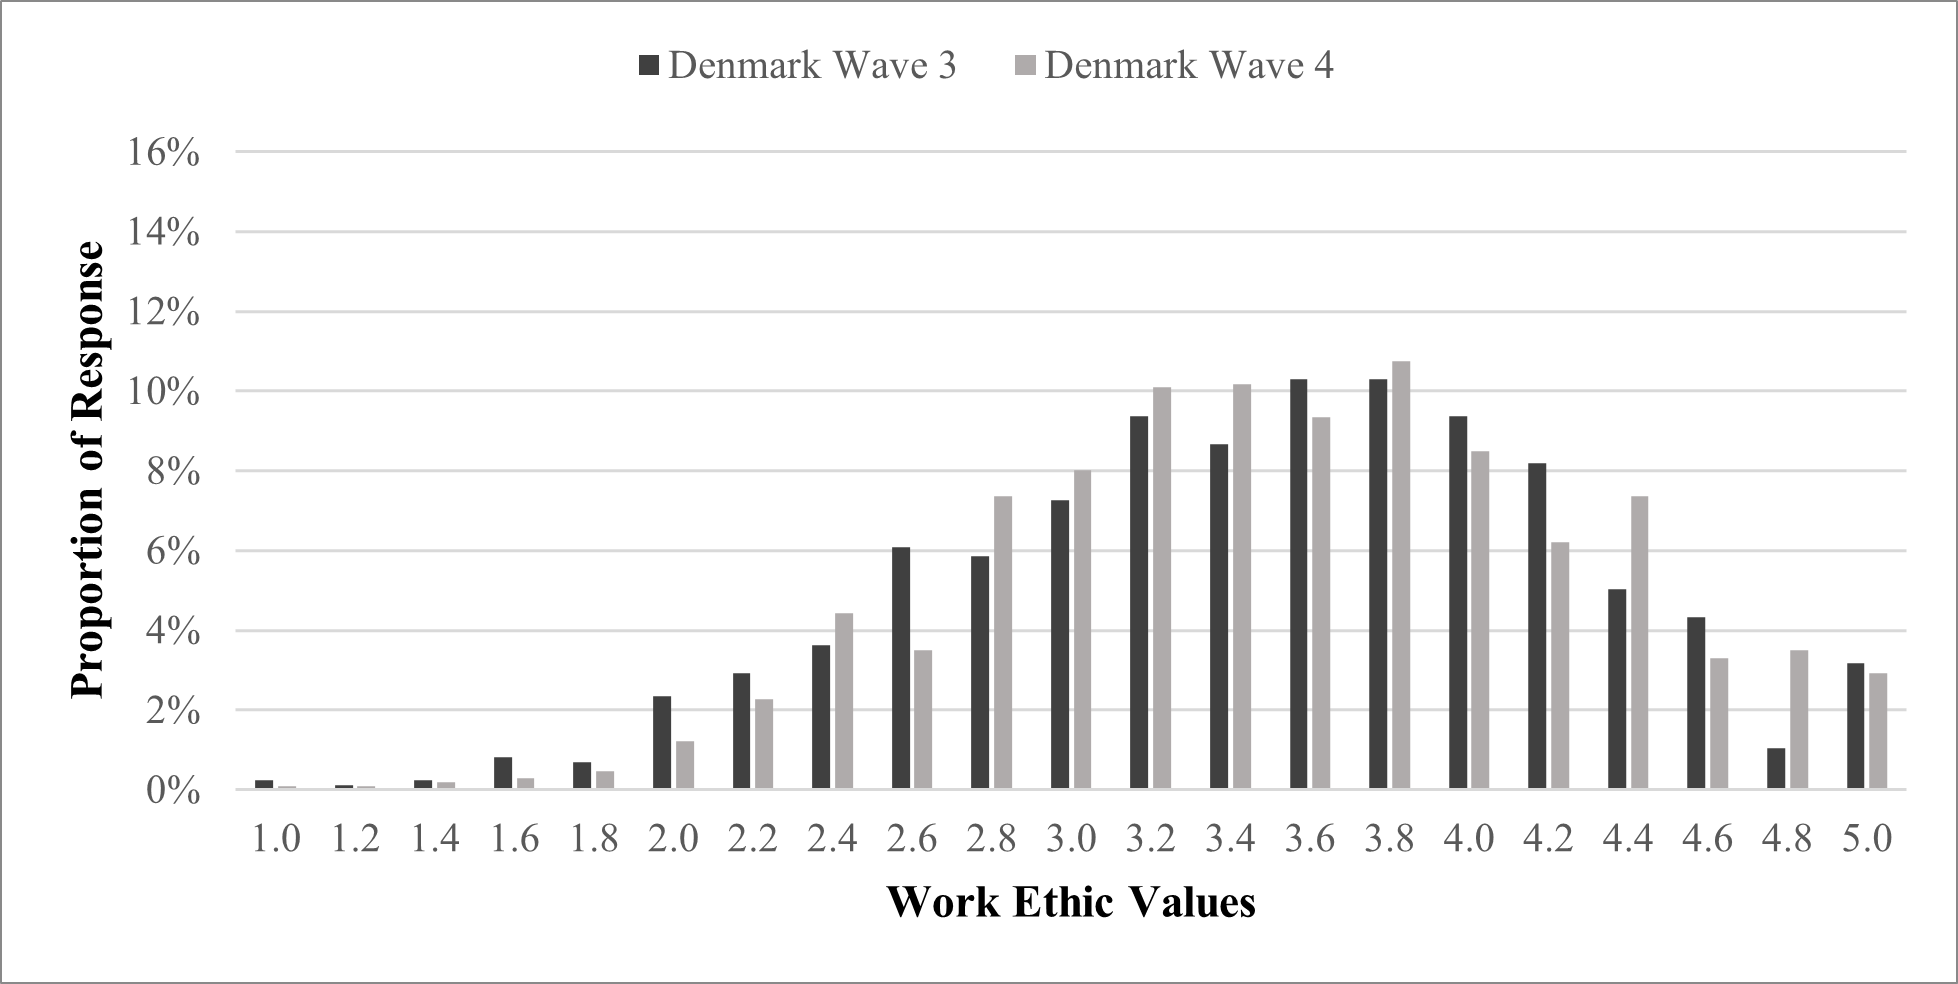
\includegraphics[width=0.95\textwidth]{figures/DenmarkQ1_5}
  \end{center}
  \caption{Distribution of Work Ethic responses for Denmark wave 3}
  \label{fig:}
\end{figure}

\begin{figure}[H]
  \begin{center}
    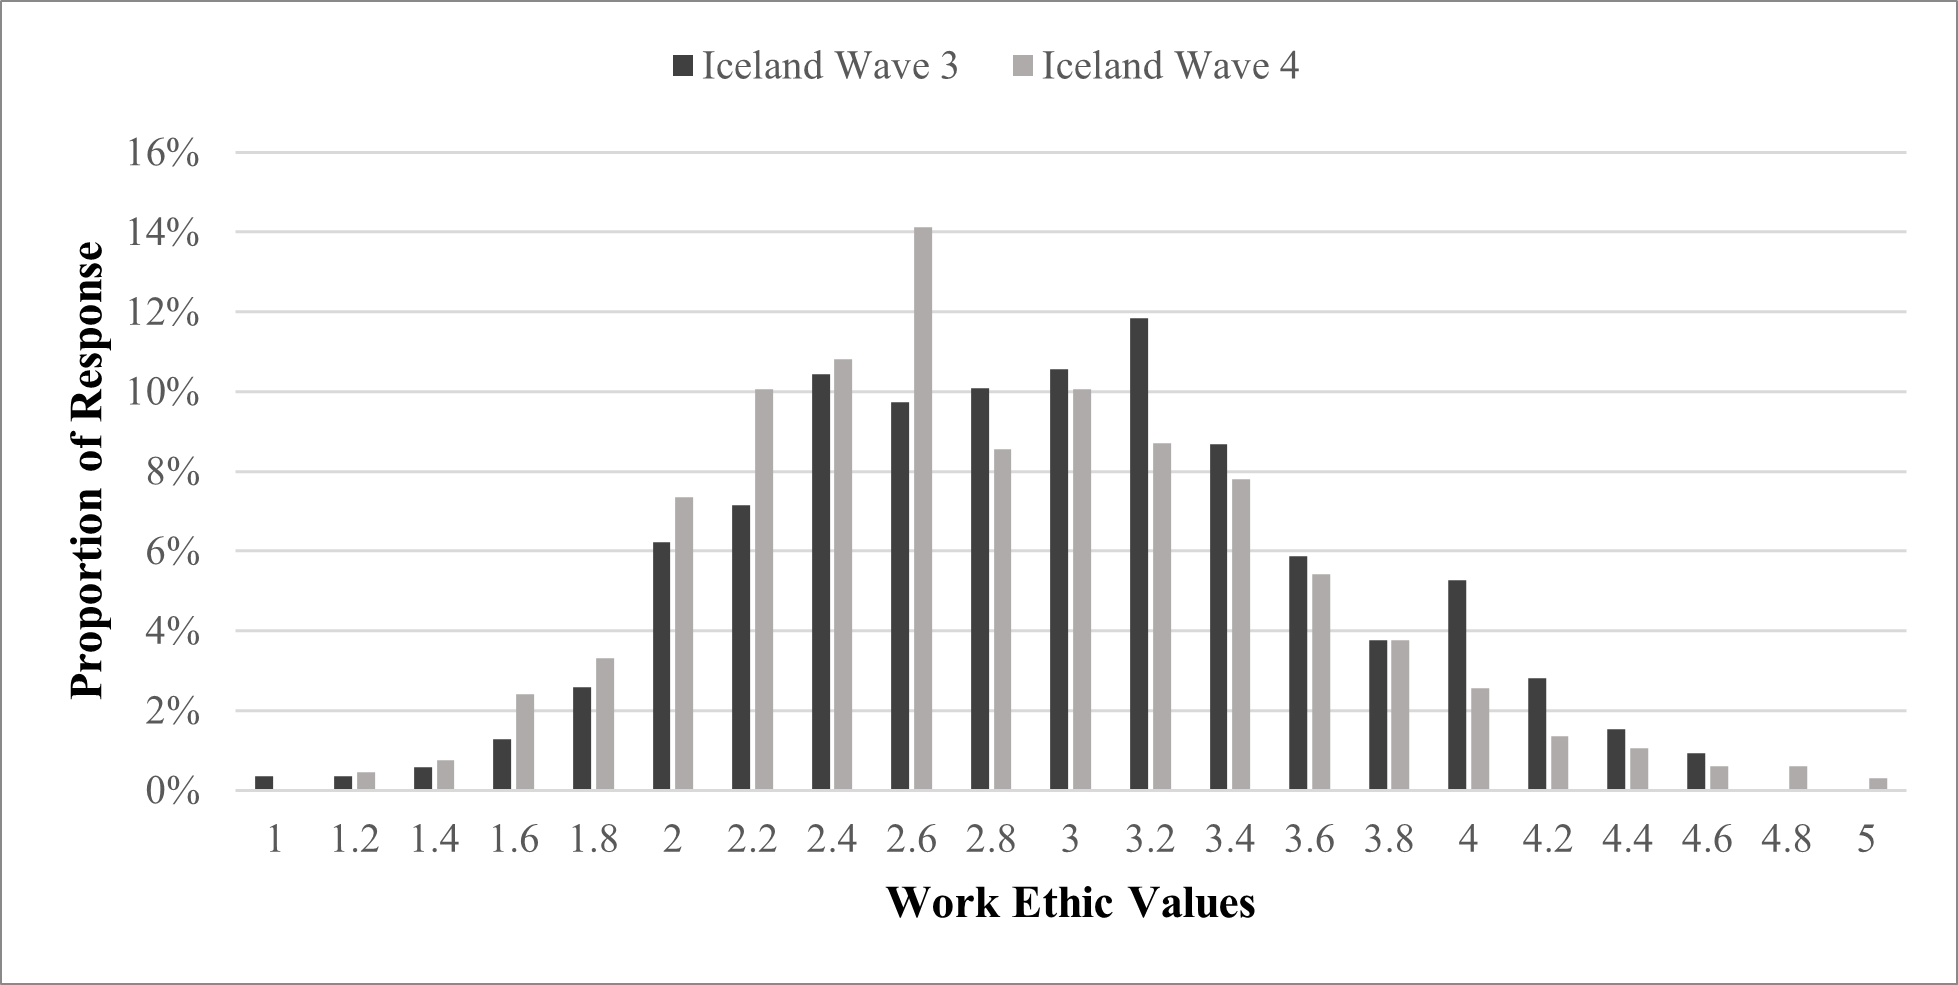
\includegraphics[width=0.95\textwidth]{figures/IcelandQ1_5}
  \end{center}
  \caption{Distribution of Work Ethic responses for Iceland wave 3}
  \label{fig:}
\end{figure}

\begin{figure}[H]
  \begin{center}
    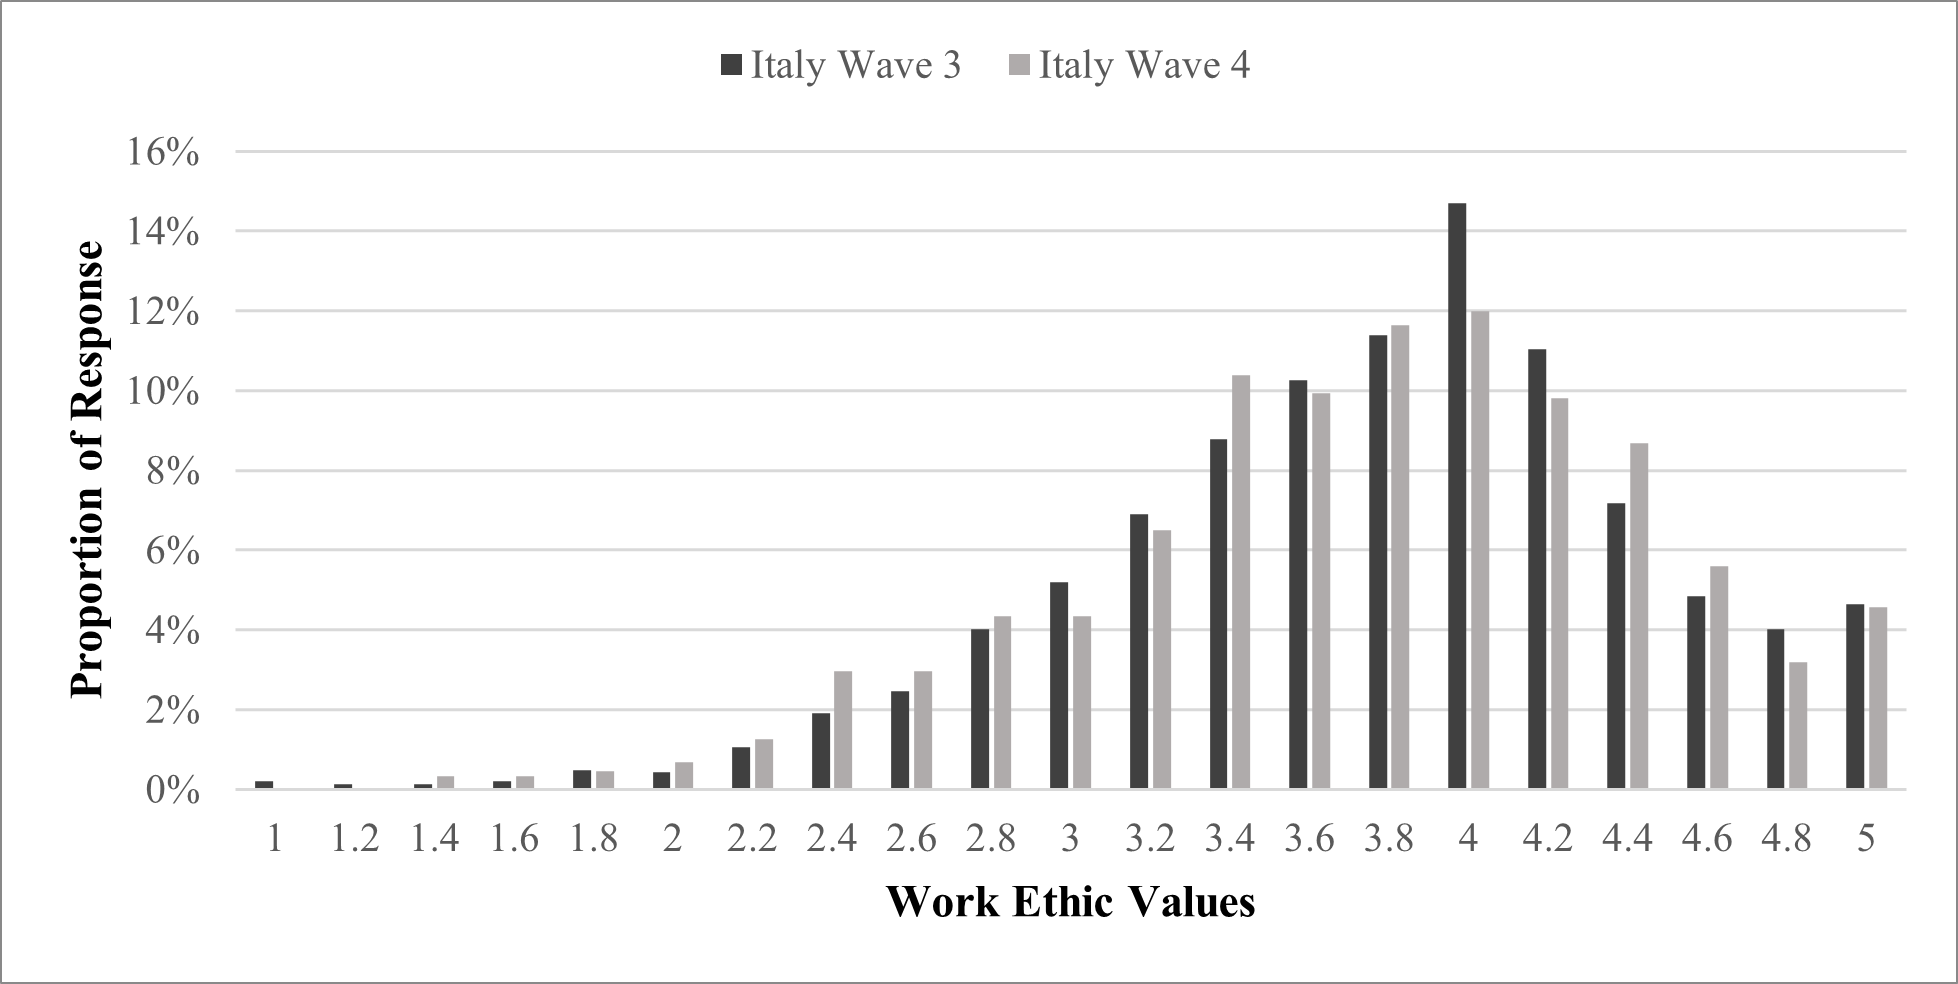
\includegraphics[width=0.95\textwidth]{figures/ItalyQ1_5}
  \end{center}
  \caption{Distribution of Work Ethic responses for Italy wave 3}
  \label{fig:}
\end{figure}



\newpage
\section*{Question 1.6}



\newpage
\bibliographystyle{agsm}
\bibliography{citations.bib}

\end{document}
